\section{Limity konvergentních posloupností}
\label{sec:limity-konvergentnich-posloupnosti}

V této sekci dokážeme, že konvergentní posloupnosti mají limitu. Opačná
implikace, tj. že posloupnosti jmajíce limitu konvergují, je téměř triviální. K
jejímu důkazu potřebujeme jen jednu vlastnost absolutní hodnoty.

\begin{lemma}{Trojúhelníková nerovnost}{trojuhelnikova-nerovnost}
 Ať $x,y \in \Q$. Pak
 \[
  |x + y| \leq |x| + |y|.
 \]
\end{lemma}
\begin{lemproof}
 Absolutní hodnota $|x+y|$ je rovna buď $x + y$ (když $x+y \geq 0$) nebo $-x-y$
 (když $x+y<0$). Zřejmě $x \leq |x|$ a $-x \leq |x|$, podobně $y \leq |y|$ a
 $-y \leq |y|$.

 Pak je ale $x + y \leq |x| + |y|$ a též $-x+(-y) \leq |x| + |y|$. Tím je důkaz
 hotov.
\end{lemproof}

\begin{remark}{}{trojuhelnikova-nerovnost}
 Název \emph{trojúhelníková} obvykle přiřazovaný
 nerovnosti~\ref{lem:trojuhelnikova-nerovnost} vyplývá z její přirozené
 geometrické interpretace. Ať $a,b,c$ jsou body v rovině. Dosazením $x = a - b$,
 $y = b - c$, dostává nerovnost~\ref{lem:trojuhelnikova-nerovnost}
 tvar
 \[
  |a - c| \leq |a - b| + |b - c|,
 \]
 tj. vzdálenost $a$ od $c$ je nanejvýš rovna součtu vzdáleností $a$ od $b$ a $b$
 od $c$ pro libovolný bod $b$.
 Vizte~\myref{obrázek}{fig:trojuhelnikova-nerovnost}.
 \begin{figure}[H]
  \centering
  \begin{tikzpicture}[scale=1.5]
   \tkzDefPoints{0/0/a,2/1/c,1.5/-0.5/b}
   \tkzDrawPolygon(a,b,c)
   \tkzDrawPoints(a,b,c)
   \tkzLabelPoint[left](a){$a$}
   \tkzLabelPoint[below](b){$b$}
   \tkzLabelPoint[right](c){$c$}

   \tkzLabelSegment[above left,xshift=1mm,yshift=-1mm](a,c){$|a - c|$}
   \tkzLabelSegment[right,yshift=-1mm](b,c){$|b - c|$}
   \tkzLabelSegment[below left,xshift=4mm](a,b){$|a - b|$}
  \end{tikzpicture}

  \caption{Trojúhelníková nerovnost}
  \label{fig:trojuhelnikova-nerovnost}
 \end{figure}
\end{remark}

Trojúhelníková nerovnost poskytuje snadné důkazy mnoha užitečných dílčích
tvrzení o posloupnostech. Příkladem je následující cvičení.

\begin{exercise}{Jednoznačnost limity}{jednoznacnost-limity}
 Dokažte, že každá posloupnost $a:\N \to \Q$ má nejvýše jednu limitu. Hint:
 použijte \hyperref[lem:trojuhelnikova-nerovnost]{trojúhelníkovou nerovnost}.
\end{exercise}

Ježto bychom však rádi dokazovali všechna tvrzení již pro reálná čísla, ukažme
si nejprve, jak se dají sčítat a násobit. Dokážeme rovněž, že $\R$ -- stejně
jako $\Q$ -- tvoří těleso. Začneme tím, že se naučíme sčítat a násobit
konvergentní posloupnosti.

Ať $a,b \in \mathcal{C}(\Q)$ jsou dvě konvergentní racionální posloupností.
Operace $+$ a $ \cdot $ na $\mathcal{C}(\Q)$ definujeme velmi přirozeně.
Zkrátka, $(a+b)(n) \coloneqq a(n) + b(n)$ a $(a \cdot b)(n) \coloneqq a(n) \cdot
b(n)$, tj. prvek na místě $n$ posloupnosti $a+b$ je součet prvků na místech $n$
posloupností $a$ a $b$. Abychom ovšem získali skutečně operace na
$\mathcal{C}(\Q)$, musíme ověřit, že $a+b$ i $a \cdot b$ jsou konvergentní.

Nechť dáno jest $\varepsilon>0$. Chceme ukázat, že umíme najít $n_0 \in \N$, aby
\[
 |(a_n + b_n) - (a_m + b_m)| < \varepsilon,
\]
kdykoli $m,n \geq n_0$. Protože jak $a$ tak $b$ konverguje, již umíme pro
libovolná $\varepsilon_a,\varepsilon_b>0$ najít $n_a$ a $n_b$ taková, že $|a_n -
a_m| < \varepsilon_a$, kdykoli $m,n \geq n_a$, a podobně $|b_n -
b_m|<\varepsilon_b$, kdykoli $m,n \geq n_b$. Položme tedy $\varepsilon_a =
\varepsilon_b \coloneqq \varepsilon / 2$ a $n_0 \coloneqq \max(n_a,n_b)$. Potom
můžeme užitím \hyperref[lem:trojuhelnikova-nerovnost]{trojúhelníkové nerovnosti}
pro $m,n \geq n_0$ odhadnout
\[
 |(a_n + b_n) - (a_m + b_m)| = |(a_n - a_m) + (b_n - b_m)| \leq |a_n - a_m| +
 |b_n - b_m| < \varepsilon_a + \varepsilon_b = \varepsilon,
\]
čili $a + b$ konverguje.

Předchozí odstavec se může snadno zdát šílenou směsicí symbolů. Ve skutečnosti
však formálně vykládá triviální úvahu. Máme najít pořadí, od kterého jsou prvky
součtu $a + b$ u sebe blíž než nějaká daná vzdálenost. Poněvadž $a$ i $b$
konvergují, stačí přeci vzít větší z pořadí, od kterých je jak rozdíl prvků $a$,
tak rozdíl prvků $b$, menší než polovina dané vzdálenosti.

Velmi obdobnou manipulaci lze provést k důkazu konvergence $a \cdot b$.
Ponecháváme jej čtenářům jako (ne zcela snadné) cvičení.

\begin{exercise}{}{}
 Dokažte, že jsou-li $a,b$ konvergentní posloupnosti racionálních čísel, pak je
 posloupnost $a \cdot b$ rovněž konvergentní. Kromě
 \hyperref[lem:trojuhelnikova-nerovnost]{trojúhelníkové nerovnosti} je zde třeba
 použít i zatím nedokázané \myref{lemma}{lem:konvergentni-omezena}.
\end{exercise}

Racionální čísla jsou přirozeně součástí reálných prostřednictvím zobrazení
\begin{equation}
 \label{eq:Q-into-R}
 \begin{split}
  \xi: \Q &\hookrightarrow \R,\\
  q &\mapsto [(q)],
 \end{split}
\end{equation}
kde $(q)$ značí posloupnost $a: n \mapsto q$ pro všechna $n \in \N$ a $[(q)]$
její třídu ekvivalence podle $ \simeq $.

\begin{warning}{}{}
 Tvrdíme pouze, že $\Q$ jsou \emph{součástí} $\R$, kde slovu \emph{součást}
 záměrně není dán rigorózní smysl. Racionální čísla totiž (aspoň po dobu naší
 dočasné \hyperref[def:realna-cisla]{definice reálných čísel}) nejsou v žádném
 smyslu podmnožinou čísel reálných.

 Matematici ale často ztotožňujeme doménu prostého zobrazení s jeho obrazem
 (neboť mezi těmito množinami vždy existuje bijekce). V tomto smyslu mohou být
 $\Q$ vnímána jako podmnožina $\R$, ztotožníme-li racionální čísla s obrazem
 zobrazení $\xi$ z \eqref{eq:Q-into-R}. Toto ztotožnění znamená vnímat
 racionální číslo $q \in \Q$ jako konvergentní posloupnost samých čísel $q$.
\end{warning}

\begin{exercise}{}{}
 Dokažte, že zobrazení $\xi$ z \eqref{eq:Q-into-R} je
 \begin{itemize}
  \item dobře definované -- tzn. že když $p = q$, pak $[(p)] = [(q)]$ -- a
  \item prosté.
 \end{itemize}
\end{exercise}

Jelikož $\Q$ je těleso, speciálně tedy obsahuje $0$ a $1$, $\R$ je
(prostřednictvím $\xi$ z \eqref{eq:Q-into-R}) obsahuje rovněž. Pro stručnost
budeme číslem $0 \in \R$ značit třídu ekvivalence posloupnosti samých nul a
číslem $1 \in \R$ třídu ekvivalence posloupnosti samých jednotek. Ověříme, že se
skutečně jedná o neutrální prvky ke sčítání a násobení.

Je třeba si rozmyslet, že pro každou posloupnost $a \in \mathcal{C}(\Q)$ platí
$a + 0 = a$ a $a \cdot 1 = a$, kde, opět, čísla $0$ a $1$ ve skutečnosti
znamenají nekonečné posloupnosti těchto čísel. Obě rovnosti jsou však zřejmé z
definice, neboť $(a+0)(n) = a_n + 0 = a_n = a(n)$ a $(a \cdot 1)(n) = a_n \cdot
1 = a_n = a(n)$ pro všechna $n \in \N$.

Konečně, rozšíříme rovněž $-$ a $^{-1}$ na $\R$. Pro libovolnou posloupnost $x
\in \mathcal{C}(\Q)$ definujeme zkrátka $(-a)(n) \coloneqq -a(n)$. S $^{-1}$ je
situace lehce komplikovanější. Totiž, pouze \textbf{nenulová} racionální čísla
mají svůj inverz k~násobení. Zde je třeba zpozorovat, že \textbf{konvergentní}
posloupnost, která by však měla nekonečně mnoho prvků nulových, už musí mít od
nějakého kroku \textbf{všechny} prvky nulové, jinak by totiž nemohla
konvergovat. Vskutku, představme si, že $a$ je posloupnost taková, že $a_n = 0$
pro nekonečně mnoho přirozených čísel $n \in \N$. Pak ale ať zvolím $n_0 \in \N$
jakkoliv, vždy existuje $m \geq n_0$ takové, že $a_m = 0$. Vezměme $n \geq n_0$
libovolné. Pokud $a_n \neq 0$, pak můžeme vzít třeba $\varepsilon \coloneqq
|a_n| / 2$ a bude platit, že $|a_n - a_m| > \varepsilon$, což je dokonalý zápor
\hyperref[def:konvergentni-posloupnost]{definice konvergence}. Z toho plyne, že
$a_n$ musí být $0$ pro $n \geq n_0$ a odtud dále, že $a \simeq 0$. Čili, pouze
posloupnosti ekvivalentní nulové posloupnosti nemají v~$\R$ inverz vzhledem k $
\cdot $.

Právě provedená úvaha nám umožňuje definovat $^{-1}$ pro posloupnosti $a \in
\mathcal{C}(\Q)$ takové, že $a \not\simeq 0$, následovně:
\[
 (a^{-1})(n) \coloneqq \begin{cases}
  a(n)^{-1},& \text{když } a(n) \neq 0,\\
  0, &\text{když } a(n) = 0.
 \end{cases}
\]
 
Je snadné uvidět, že $-a$ je inverzem k $a$ vzhledem k $+$ a $a^{-1}$ je
inverzem k $a \neq 0$ vzhledem k $ \cdot $. Vskutku, máme
\[
 (a + (-a))(n) = a_n + (-a_n) = 0,
\]
tedy v tomto případě je $(a + (-a))$ přímo \textbf{rovna} nulové posloupnosti. V
případě $^{-1}$ dostáváme pro $a \not\simeq 0$
\[
 (a \cdot a^{-1})(n) = \begin{cases}
  a_n \cdot a_n^{-1} = 1,& \text{když } a_n \neq 0,\\
  a_n \cdot 0 = 0,& \text{když } a_n = 0.
 \end{cases}
\]
Ergo, $a \cdot a^{-1}$ je rovna posloupnosti samých jedniček, až na konečně
mnoho nul, protože, jak jsme si již rozmysleli, $a$ nemůže mít nekonečně $0$ a
zároveň nebýt v relaci $ \simeq $ s nulovou posloupností, jinak by nebyla
konvergentní. To však přesně znamená, že $a \cdot a^{-1} \simeq 1$, čili $[a]
\cdot [a^{-1}] = [1]$.

Shrneme-li řád předchozích úvah, získáme oprávnění tvrdit, že
\[
 (\R,+,-,[(0)], \cdot,^{-1},[(1)])
\]
je těleso. Tento fakt je do budoucna pochopitelně zásadní; teď se však můžeme
těšit znalostí, že jsme přechodem od $\Q$ k $\R$ neztratili symetrické rysy
původní množiny.

Přikročmež již však k důkazu existence limity každé konvergentní posloupnosti.
Fakt, že existence limity implikuje konvergenci, plyne přímo z
\hyperref[lem:trojuhelnikova-nerovnost]{trojúhelníkové nerovnosti}.

\begin{lemma}{}{limita-konvergence}
 Každá posloupnost majíc limitu je konvergentní.
\end{lemma}
\begin{lemproof}
 Ať $a:\N \to \Q$ je posloupnost s limitou $L$. Pak pro každé $\varepsilon_L>0$
 existuje $n_L \in \N$ takové, že $|a_n - L| < \varepsilon_L$ pro všechna $n
 \geq n_L$.

 Ať je dáno $\varepsilon>0$. Chceme ukázat, že $|a_m - a_n| < \varepsilon$ pro
 všechna $m,n$ větší než vhodné $n_0 \in \N$. Položme tedy $n_0 \coloneqq n_L$ a
 $\varepsilon_L \coloneqq \varepsilon / 2$. Potom pro všechna $m,n \geq n_0 =
 n_L$ máme
 \[
  |a_m - a_n| = |a_m - a_n - L + L| = |(a_n - L) + (L - a_m)| \leq |a_n - L| +
  |L - a_m| < \varepsilon_L + \varepsilon_L = \varepsilon,
 \]
 čili $a$ konverguje.
\end{lemproof}

\subsection{Úplnost reálných čísel}
\label{ssec:uplnost-realnych-cisel}

K důkazu existence limity každé konvergentní posloupnosti potřebujeme
prozpytovat vztah racionálních a reálných čísel podrobněji. Konkrétně
potřebujeme ukázat, že $\Q$ jsou tzv. \emph{hustá} v $\R$, tj. že ke každému
reálnému číslu existuje racionální číslo, které je mu nekonečně blízko. Zde jsme
opět implicitně ztotožnili racionální čísla s třídami ekvivalence konstantních
posloupností. Na základě toho budeme totiž moci tvrdit, že reálná čísla jsou
tzv. \emph{úplná}, což přesně znamená, že každá konvergentní posloupnost
reálných čísel má reálnou limitu.

Nejprve si ovšem musíme rozmyslet, co vlastně míníme posloupností
\emph{reálných} čísel. Pochopitelně, zobrazení $x:\N \to \R$ poskytuje validní
definici, ale uvědomme sobě, že teď vlastně uvažujeme posloupnosti, jejichž
prvky jsou třídy ekvivalence konvergentních racionálních posloupností.

Abychom směli hovořit o konvergentních \emph{reálných} posloupnostech, rozšíříme
absolutní hodnotu $| \cdot |$ z $\Q$ na $\R$ zkrátka předpisem $|[(x_n)]|
\coloneqq [(|x_n|)]$ pro $(x_n) \in \mathcal{C}(\Q)$. Napíšeme-li tedy $|x| \leq
K$ pro reálná čísla $x,K \in \R$, pak tím doslova myslíme $[(|x_n|)] \leq
[(K_n)]$, což ale \textbf{neznamená} $|x_n| \leq K_n$ pro všechna $n \in \N$,
kde $x_n,K_n$ jsou nyní již čísla ryze rozumná čili racionální, anobrž $|x_n| >
K_n$ jen pro \textbf{konečně mnoho} $n \in \N$.

\begin{warning}{}{}
 Důležitá myšlenka, již je dlužno snovat v srdci při práci s třídami ekvivalence
 konvergentních posloupností, je ta, že při porovnávání dvou tříd nás nezajímá
 libovolný \textbf{konečný počet} jejich prvních prvků.

 Například, vztah $x = y$ pro $x,y \in \R$ znamená, že $x_n = y_n$ pro každé $n
 \in \N$ až na libovolný konečný počet prvních přirozených čísel. To se lépe
 vyjadřuje pomocí negace. Je snazší říct, že $x = y$, když $x_n \neq y_n$ pro
 jenom konečně mnoho $n \in \N$.
\end{warning}

Rozepíšeme-li si tedy podrobně, co znamená, že je posloupnost $x:\N \to \R$
konvergentní, dostaneme pro dané $\varepsilon>0$, vhodné $n_0 \in \N$ a $m,n
\geq n_0$ nerovnost $|x_n - x_m| < \varepsilon$. Ovšem, $x_n$ i $x_m$ jsou samy
o sobě třídy ekvivalence konvergentních \textbf{posloupností} racionálních
čísel, tedy poslední nerovnost plně rozepsána dí
\[
 |[((x_n)_{k} - (x_m)_{k})_{k=0}^{\infty}]| < \varepsilon,
\]
což lze rovněž vyjádřit tak, že
\[
 |(x_n)_k - (x_m)_k| \geq \varepsilon
\]
jen pro konečně mnoho $k \in \N$.

Nepřináší však žádný hmotný užitek nad konvergencí reálných posloupností
uvažovat takto složitě. Čtenáři dobře učiní, uvědomí-li si plný význam
předchozího odstavce, ovšem zůstanou-li věrni intuitivnímu vnímání výrazu $|x -
y|$ jako \uv{vzdálenosti} čísel $x$ a $y$.

\begin{definition}{Omezená posloupnost}{omezena-posloupnost}
 Řekneme, že posloupnost $x:\N \to \R$ je \emph{omezená}, když existuje $K \in
 \R$ takové, že $|x_n| \leq K$ pro všechna $n \in \N$. Píšeme $|x| \leq K$.
\end{definition}

\begin{lemma}{}{konvergentni-omezena}
 Každá konvergentní posloupnost $x:\N \to \R$ je omezená.
\end{lemma}
\begin{lemproof}
 Ať je $\varepsilon>0$ dáno. Z \hyperref[def:konvergentni-posloupnost]{definice
 konvergence} nalezneme $n_0 \in \N$ takové, že pro každé $m,n \geq n_0$ je
 $|x_m - x_n| < \varepsilon$. Speciálně tedy pro každé $n \geq n_0$ platí
 \[
  |x_n| = |x_n - x_{n_0} + x_{n_0}| \leq |x_n - x_{n_0}| + |x_{n_0}| <
  \varepsilon + |x_{n_0}|,
 \]
 tudíž všechny členy posloupnosti s pořadím větším než $n_0$ jsou omezeny číslem
 $\varepsilon + |x_{n_0}|$. Ovšem, členů posloupnosti s pořadím menším než $n_0$
 je konečně mnoho, a tedy z nich můžeme vzít ten největší -- nazvěme ho $s$.
 Položíme-li $K \coloneqq \max(s,\varepsilon + |x_{n_0}|)$, pak $|x_n| \leq K$
 pro každé $n \in \N$, čili $x$ je omezená číslem $K$.
\end{lemproof}

\begin{proposition}{Hustota $\Q$ v $\R$}{hustota-q-v-r}
 Množina racionálních čísel $\Q$ je hustá v $\R$, tj. ke každému $x \in \R$ a
 každému $\varepsilon>0$ existuje $r \in \Q$ takové, že $|x-r|<\varepsilon$.
\end{proposition}
\begin{propproof}
 Ať $\varepsilon>0$ je dáno a označme $x \coloneqq [(x_n)]$, $(x_n) \in
 \mathcal{C}(\Q)$. Najdeme $n_0 \in \N$ takové, že $ \forall m,n \geq n_0$ je
 $|x_m - x_n|<\varepsilon$. Zvolme $r \coloneqq x_{n_0} \in \Q$. Pak ovšem máme
 \[
  |x_n - r| = |x_n - x_{n_0}| < \varepsilon
 \]
 pro všechna $n \geq n_0$. To přesně znamená, že $|x - r| < \varepsilon$.
\end{propproof}

\begin{lemma}{}{limita-racionalni-posloupnosti}
 Ať $a:\N \to \Q$ je konvergentní posloupnost racionálních čísel. Pak $\lim a =
 [(a)]$.
\end{lemma}
\begin{lemproof}
 Položme $x \coloneqq [(a)]$. Ať je dáno $\varepsilon>0$. Protože $a$ je
 konvergentní, nalezneme $n_0 \in \N$, že $|a_m - a_n|<\varepsilon$ pro všechna
 $m,n \geq n_0$. Potom ale $|a_n - x|<\varepsilon$ pro všechna $n \geq n_0$, což
 z~\hyperref[def:limita-posloupnosti]{definice} znamená, že $\lim_{} a = x$.
\end{lemproof}

\begin{corollary}{$\R$ jsou úplná}{r-jsou-uplna}
 Každá konvergentní reálná posloupnost $x:\N \to \R$ má limitu v $\R$.
\end{corollary}
\begin{corproof}
 Ať $a:\N \to \Q$ je racionální posloupnost taková, že $|x_n - a_n|<1/n$ pro
 všechna $n \in \N$. Tu nalezneme opakovaným použitím
 \myref{tvrzení}{prop:hustota-q-v-r} pro $\varepsilon \coloneqq 1 / n$ a $x
 \coloneqq x_n$. Ukážeme nejprve, že $a$ je konvergentní. Ať je dáno
 $\varepsilon>0$. Zvolme $n_1$ takové, že $ \forall m,n \geq n_1$ platí $1 / m +
 1 / n < \varepsilon$. Dále, $x$ je konvergentní z předpokladu. Čili, pro každé
 $\varepsilon_x>0$ nalezneme $n_2 \in \N$ takové, že $ \forall m,n \geq n_2$
 máme $|x_n - x_m|<\varepsilon_x$. Volme tedy speciálně
 \[
  \varepsilon_x \coloneqq \varepsilon - \frac{1}{m} - \frac{1}{n}.
 \]
 a $n_0 \coloneqq \max(n_1,n_2)$. Potom pro všechna $m,n \geq n_0$ platí
 nerovnosti
 \begin{align*}
  |a_n - a_m| &= |a_n - a_m - x_n + x_n| \leq |a_n - x_n| + |x_n - a_m| = |a_n -
  x_n| + |x_n - a_m - x_m + x_m| \\
              & \leq |a_n - x_n| + |x_n - x_m| + |x_m - a_m| < \frac{1}{n} +
              \varepsilon_x + \frac{1}{m} = \varepsilon,
 \end{align*}
 tedy $a$ konverguje.

 Jistě platí $\lim_{} x - a = 0$, neboť pro každé $\varepsilon>0$ lze najít
 $n \in \N$ takové, že $1 / n < \varepsilon$. Odtud plyne, že $x$ má limitu
 právě tehdy, když $a$ má limitu. Ovšem, podle
 \myref{lemmatu}{lem:limita-racionalni-posloupnosti} má $a$ limitu $[(a)] \in
 \R$. Tím je důkaz hotov.
\end{corproof}

\begin{corollary}{}{}
 Platí
 \[
  \R \cong \{\lim_{} a \mid a \in \mathcal{C}(\Q)\},
 \]
 čili reálná čísla jsou přesně limity všech konvergentních racionálních
 posloupností.
\end{corollary}
\begin{corproof}
 Zkonstruujeme bijekci $f: \R \to \{\lim_{} a \mid a \in \mathcal{C}(\Q)\}$.
 Vezměme $x \in \R$. Pak z definice existuje konvergentní racionální posloupnost
 $a \in \mathcal{C}(\Q)$ taková, že $x = [a]$. Podle
 \myref{lemmatu}{lem:limita-racionalni-posloupnosti} má $a$ limitu v $\R$.
 Definujme tedy $f(x) \coloneqq \lim_{} a$.

 Ověříme, že je $f$ dobře definované, prosté a na.

 Nejprve musíme ukázat, že $f(x)$ nezávisí na volbě konkrétní posloupnosti $a$ z
 třídy ekvivalence $[a]$. Ať tedy $b \simeq a$ a označme $L_a \coloneqq \lim_{}
 a, L_b \coloneqq \lim_{} b$. Pak pro každé $\varepsilon>0$ existuje $n_0 \in
 \N$ takové, že $ \forall n \geq n_0$ platí tři nerovnosti:
 \[
  |a_n-b_n|<\varepsilon, \quad |a_n-L_a|<\varepsilon, \quad
  |b_n-L_b|<\varepsilon.
 \]
 Velmi obdobnou úpravou jako v důkaze \myref{důsledku}{cor:r-jsou-uplna}
 dostaneme,
 že
 \[
  |L_a - L_b| \leq |L_a - a_n| + |a_n - b_n| + |b_n - L_b| < 3\varepsilon,
 \]
 odkud $L_a = L_b$, neboť $L_a,L_b$ jsou třídy ekvivalence konvergentních
 posloupností. Společně s faktem, že každá konvergentní posloupnost má přesně
 jednu limitu (\myref{cvičení}{exer:jednoznacnost-limity}), plyne z~předchozí
 úvahy, že $f$ je dobře definováno.

 Dokážeme, že $f$ je prosté. To je snadné, neboť pokud $[a] = [b]$, neboli $a
 \simeq b$, potom $\lim_{} a = \lim_{} b$, což jsme již vlastně dokázali v
 odstavci výše.

 Nakonec zbývá ověřit, že $f$ je na. Ať tedy $L \coloneqq \lim a$ pro nějakou $a
 \in \mathcal{C}(\Q)$. Potom ovšem $[(a)] \in \R$ a podle
 \myref{lemmatu}{lem:limita-racionalni-posloupnosti} platí $\lim a = [(a)]$. To
 ovšem přesně znamená, že $f([(a)]) = L$.

 Tím je důkaz hotov.
\end{corproof}
